\documentclass[tikz,border=3.14mm]{standalone}
\usepackage{amsmath}
\usetikzlibrary{arrows.meta}

\begin{document}

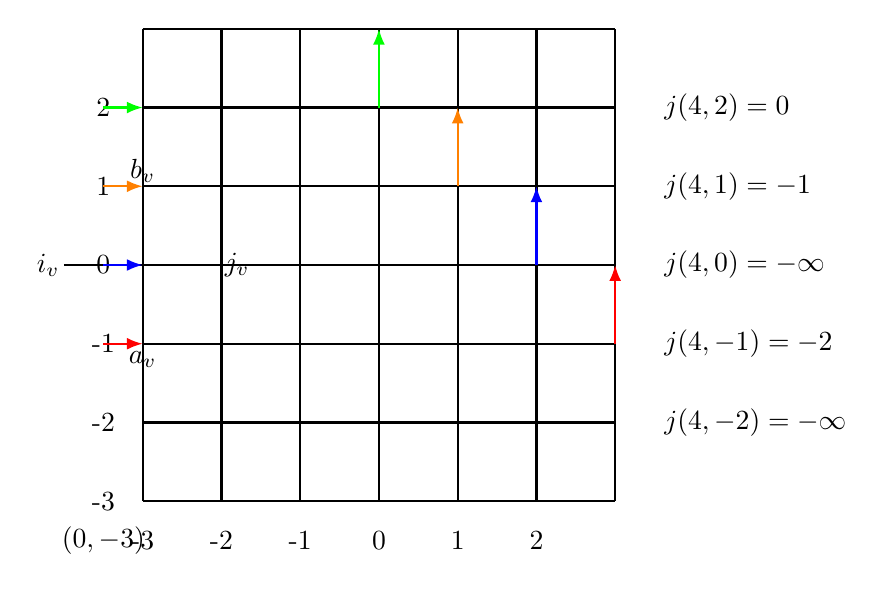
\begin{tikzpicture}

% Left diagram: labels for the arrow configuration at a vertex
\draw[thick] (-1,0) -- (1,0);
\draw[thick] (0,-1) -- (0,1);
\node at (-1.2,0) {$i_v$};
\node at (1.2,0) {$j_v$};
\node at (0,-1.2) {$a_v$};
\node at (0,1.2) {$b_v$};

% Right diagram: sample configuration of the colored stochastic six-vertex model
\begin{scope}[shift={(3,0)}]
    \draw[step=1cm,thick] (-3,-3) grid (3,3);
    \foreach \x in {-3,-2,-1,0,1,2} {
        \node at (\x,-3.5) {\x};
        \node at (-3.5,\x) {\x};
    }

    \node at (-3.5,-3.5) {$(0,-3)$};
    
    % Arrows with colors
    \draw[-{Latex[length=2mm]},thick,red] (-3.5,-1) -- (-3,-1);
    \draw[-{Latex[length=2mm]},thick,blue] (-3.5,0) -- (-3,0);
    \draw[-{Latex[length=2mm]},thick,orange] (-3.5,1) -- (-3,1);
    \draw[-{Latex[length=2mm]},thick,green] (-3.5,2) -- (-3,2);
    
    \draw[-{Latex[length=2mm]},thick,green] (0,2) -- (0,3);
    \draw[-{Latex[length=2mm]},thick,orange] (1,1) -- (1,2);
    \draw[-{Latex[length=2mm]},thick,blue] (2,0) -- (2,1);
    \draw[-{Latex[length=2mm]},thick,red] (3,-1) -- (3,0);

    % Labels
    \node[right] at (3.5,2) {$j(4,2) = 0$};
    \node[right] at (3.5,1) {$j(4,1) = -1$};
    \node[right] at (3.5,0) {$j(4,0) = -\infty$};
    \node[right] at (3.5,-1) {$j(4,-1) = -2$};
    \node[right] at (3.5,-2) {$j(4,-2) = -\infty$};
    
\end{scope}

\end{tikzpicture}

\end{document}